%% ----------------------------------------------------------------
%% SETTINGS
%% ----------------------------------------------------------------
\documentclass[../et.tex]{subfiles}

%% ----------------------------------------------------------------
%% BEGIN
%% ----------------------------------------------------------------
\begin{document}

%% ----------------------------------------------------------------
%% DOCUMENT
%% ----------------------------------------------------------------
Para la implementación del lazo de control de corriente en el multiplicador y la adquisición de la señal entregada por la sonda de corriente a caracterizar, se utilizará un conversor analógico digital.

Se utilizará el integrado ADS1174IPAPT. El esquemático para la conexión del mismo, por su complejidad, fue dividido en secciones.

%% ----------------------------------------------------------------
\subsubsection{Alimentación}
%% ----------------------------------------------------------------
Este dispositivo, necesita tres fuentes de alimentación separadas: \SI{5}{V}, \SI{3.3}{V} y \SI{1.8}{V}. Debido a indicaciones del fabricante, se agregó un capacitor de desacople de \SI{10}{\micro F} entre cada entrada y masa, como se puede ver en la \autoref{fig:adc-supply}

\begin{figure}[!htbp]
  \centering
  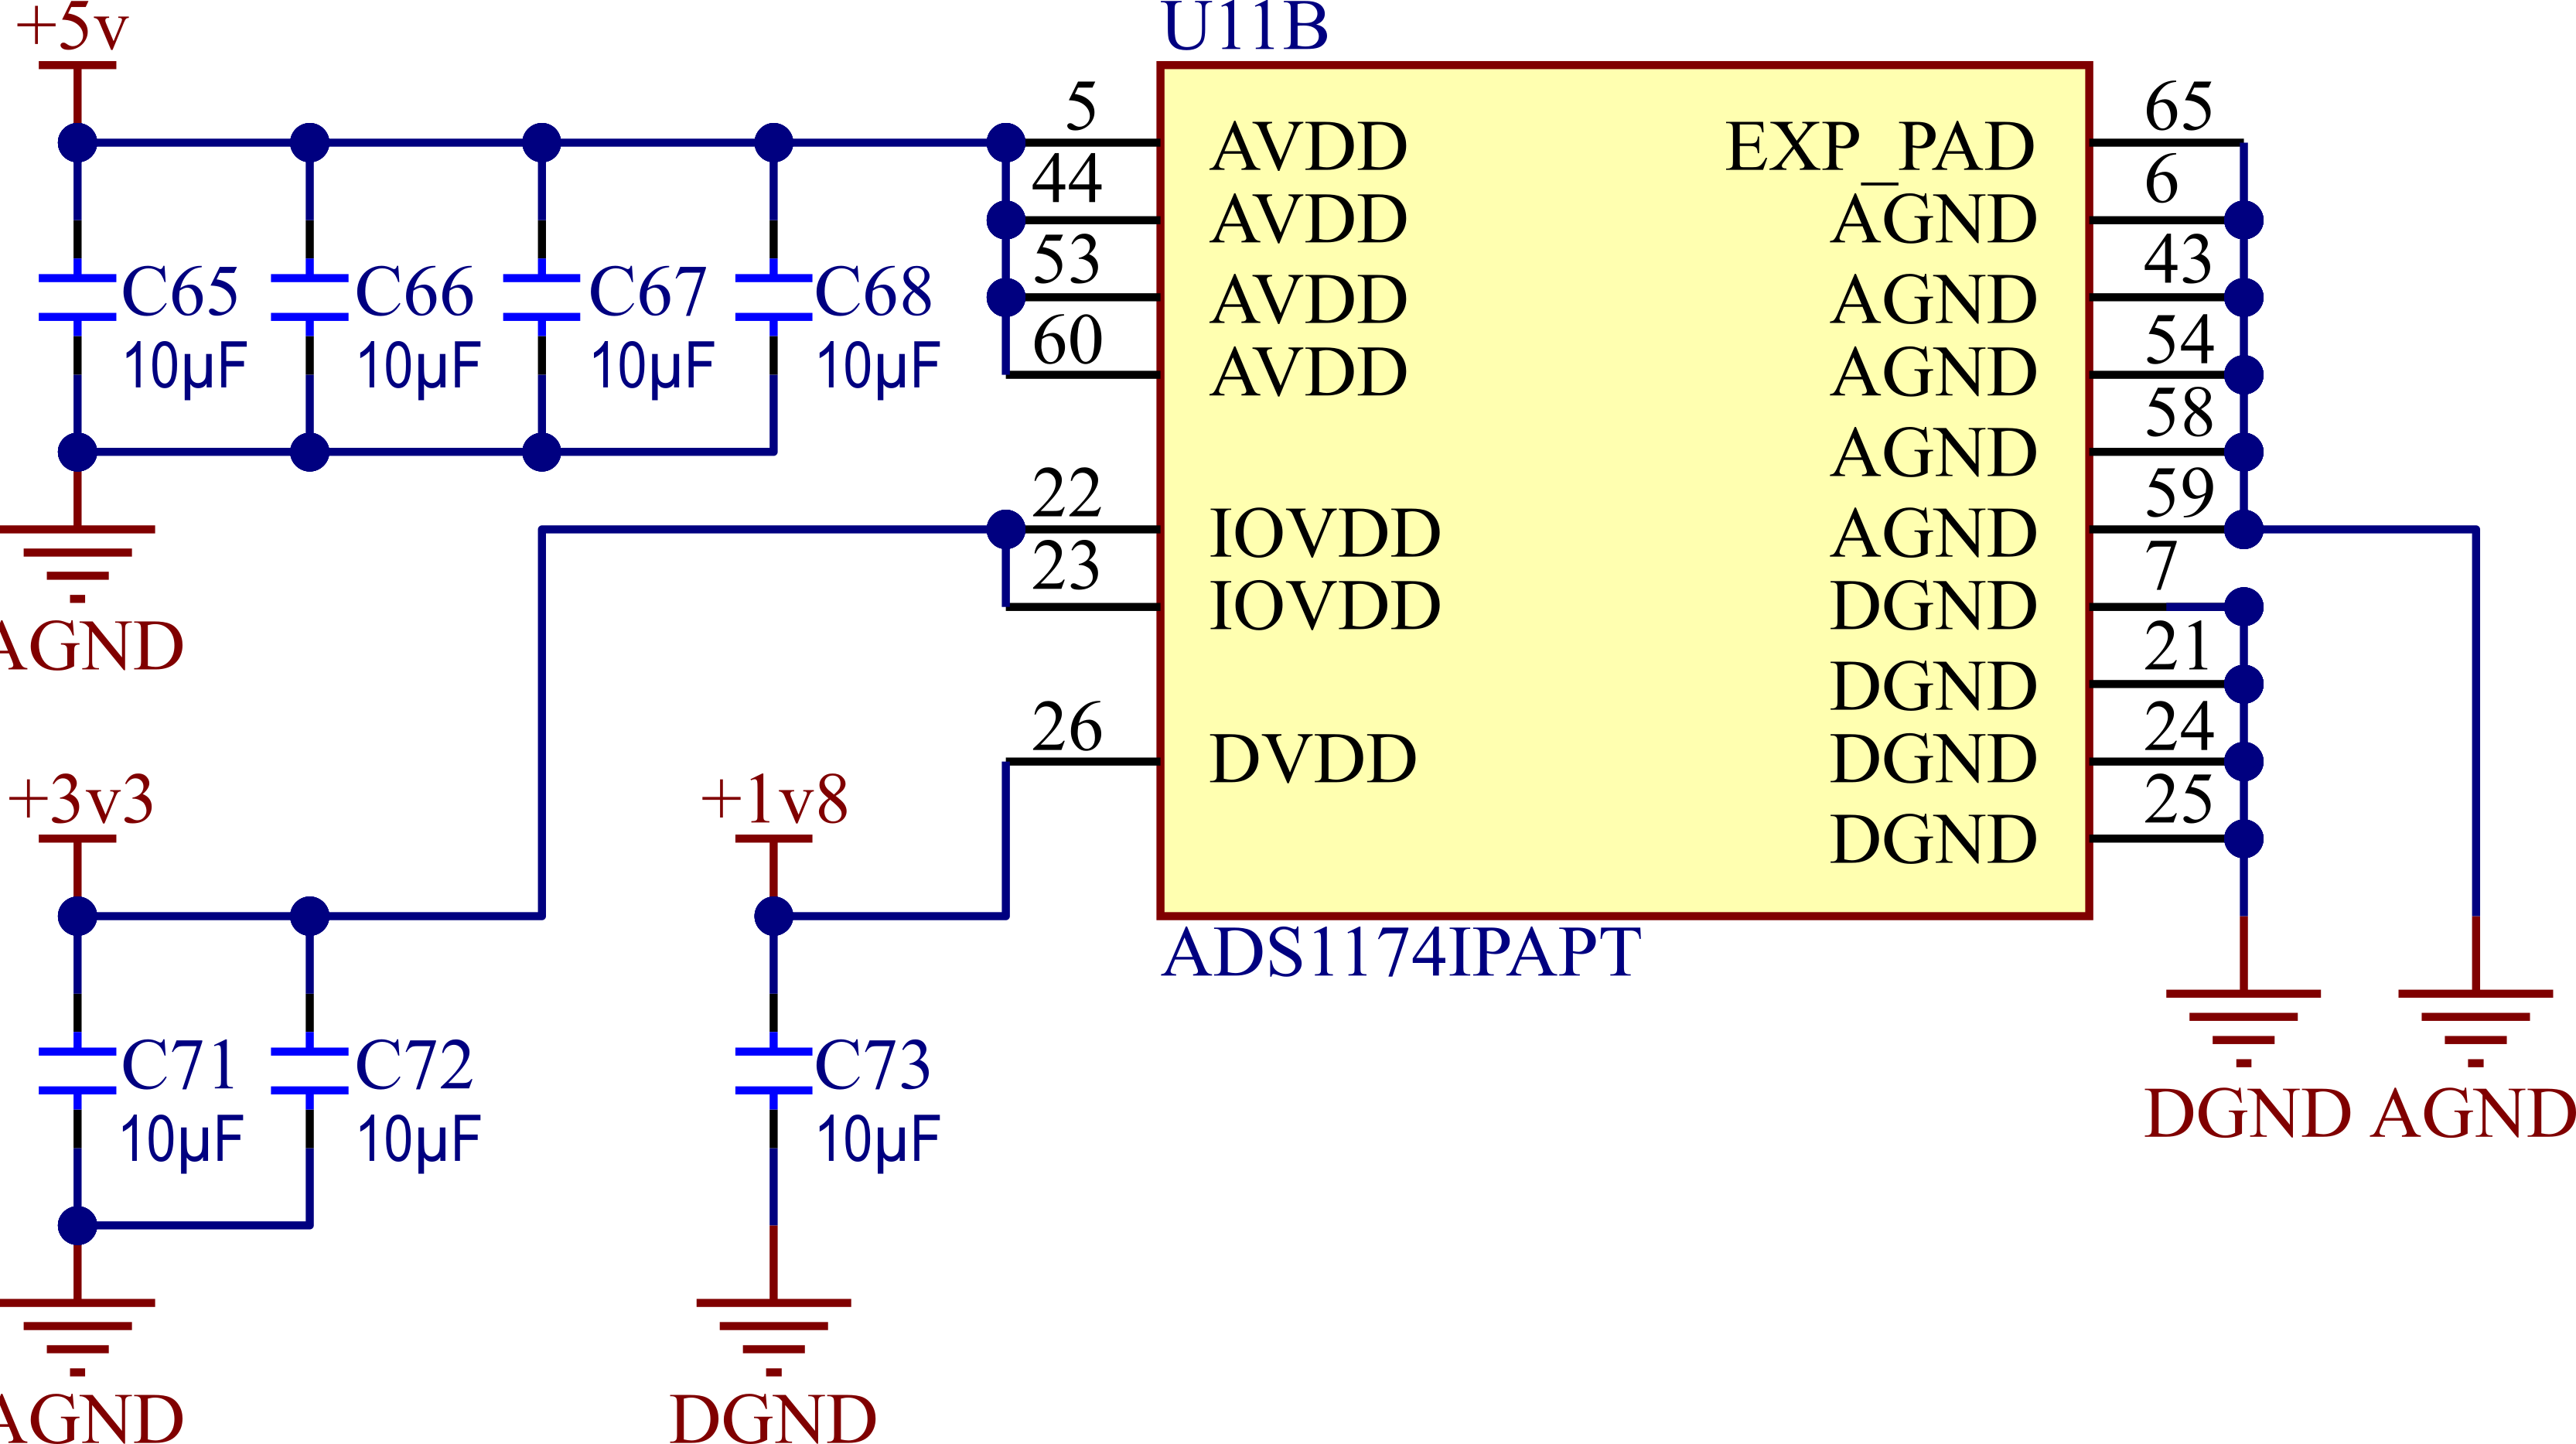
\includegraphics[width=0.6\textwidth]{../images/adc-supply.png}
  \caption{Alimentación del ADC}
  \label{fig:adc-supply}
\end{figure}

%% ----------------------------------------------------------------
\subsubsection{Entradas analógicas}
%% ----------------------------------------------------------------
En el caso de las entradas analógicas, se colocó un capacitor cerámico de \SI{2.2}{nF} entre cada entrada diferencial, por indicación del fabricante para mejorar la performance del sistema. Además, se colocaron las cuatro entradas superiores (AINP4-AINP8) a masa, ya que éstas sólo están habilitadas en la versión de 8 canales del integrado. En esta etapa se incluyó también la tensión de referencia, la cual dictará el fondo de escala del dispositivo. El esquemático resultante se puede ver en la \autoref{fig:adc-inputs}.

\begin{figure}[!htbp]
  \centering
  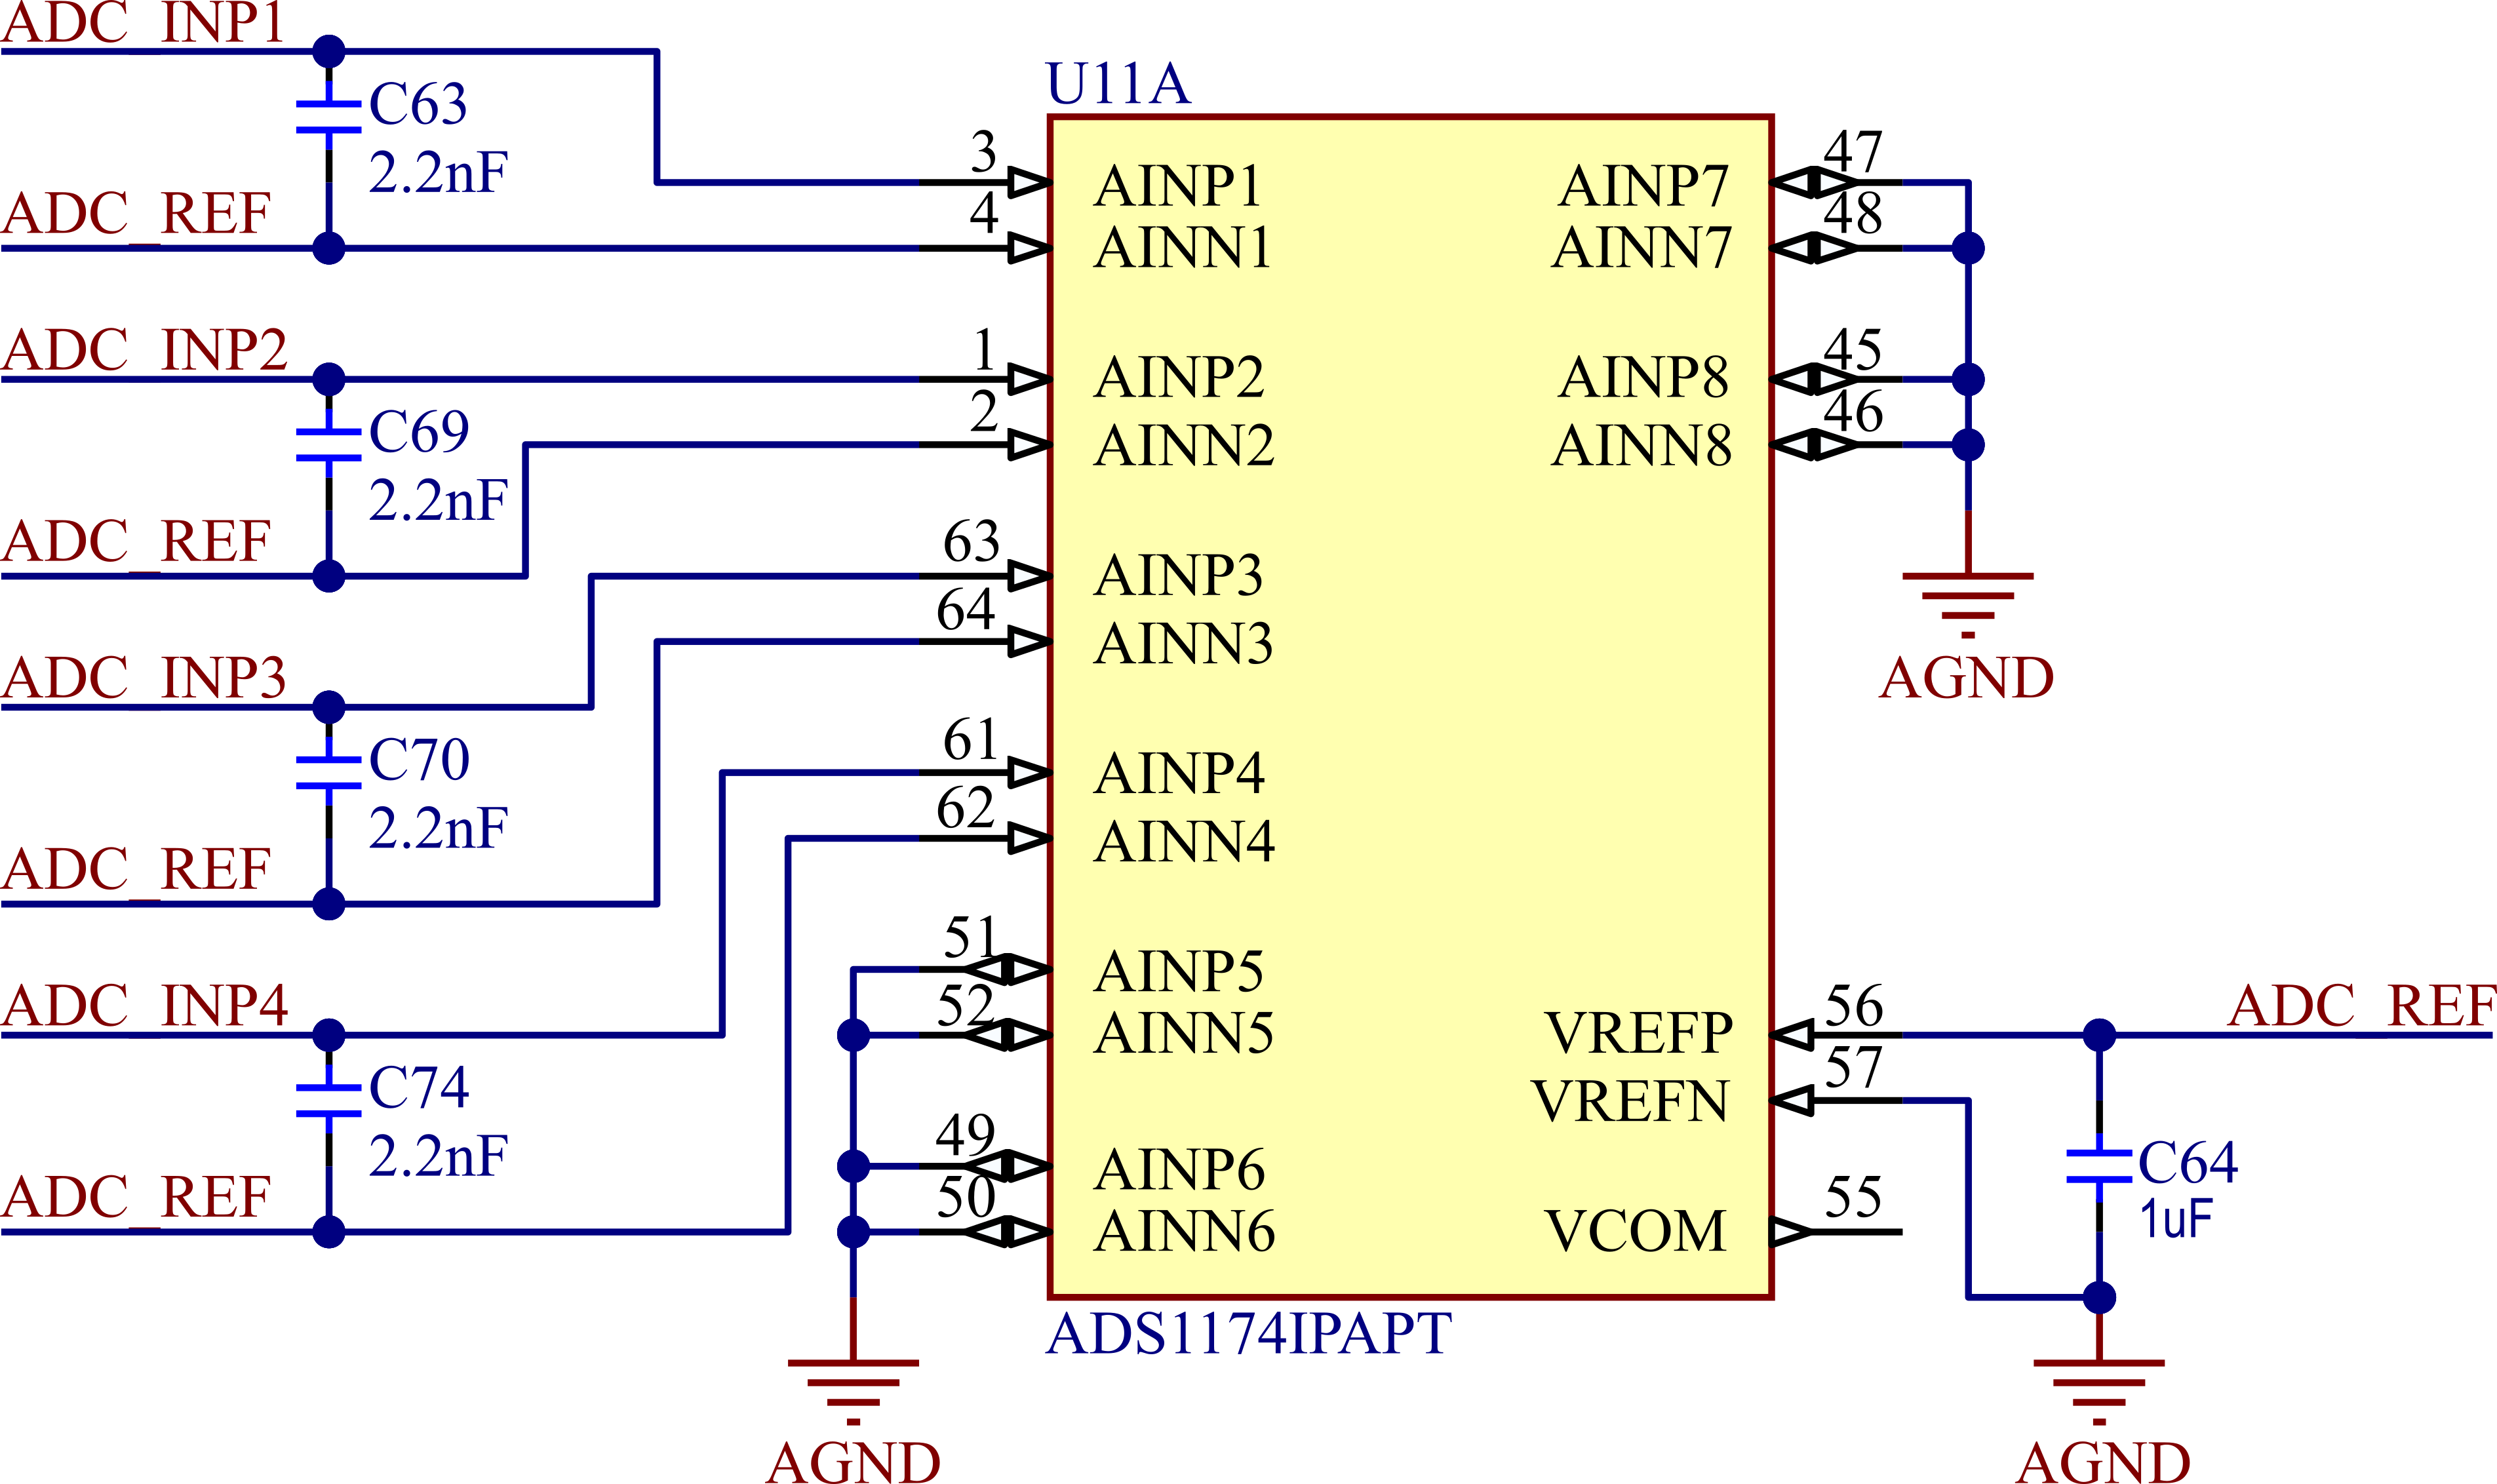
\includegraphics[width=0.6\textwidth]{../images/adc-inputs.png}
  \caption{Entradas analógicas del ADC}
  \label{fig:adc-inputs}
\end{figure}

%% ----------------------------------------------------------------
\subsubsection{Entradas y salidas digitales}
%% ----------------------------------------------------------------
Siguiendo las indicaciones del fabricante, se conectó el pin DOUT1 a la entrada SPI\_MISO (Master Input Slave Output) del microcontrolador, terminando la conexión con una resistencia de \SI{100}{\ohm} para adaptación de impedancias. Se conectó también SPCK al clock del SPI del microcontrolador y CLK al clock generado por el PWM del microcontrolador. El pin de DRDY (data ready) se ha conectado a una entrada GPIO del microcontrolador.

El funcionamiento de la interfaz SPI es el siguiente. Una vez que el ADC tiene los datos listos, genera una interrupción en el microcontrolador a través del pin de DRDY. El microcontrolador así comienza a generar el clock del SPI y el ADC envía los datos. En la \autoref{fig:adc-spi-tdm} se puede observar una descripción gráfica del funcionamiento descripto.

\begin{figure}[!htbp]
  \centering
  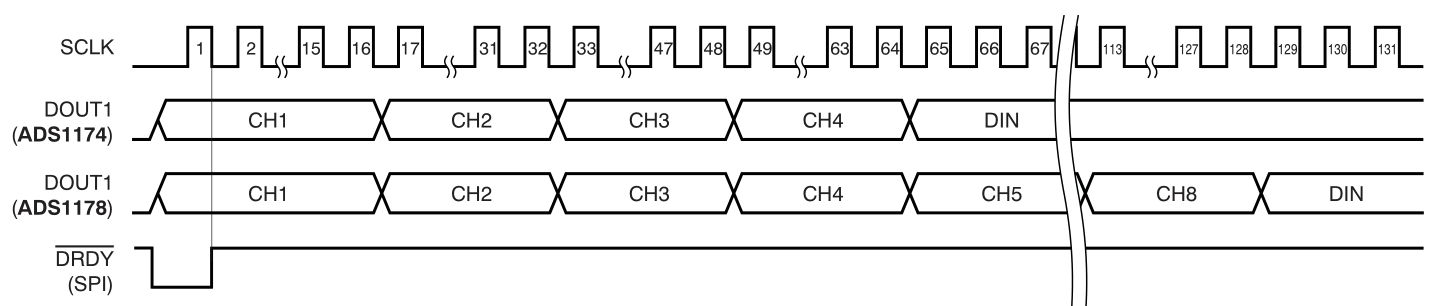
\includegraphics[scale=0.4]{../images/adc-spi-tdm.png}
  \caption{Diagrama de tiempo de envío de datos del ADC en modo TDM}
  \label{fig:adc-spi-tdm}
\end{figure}

%% ----------------------------------------------------------------
\subsubsection{Modos de salida de datos}
%% ----------------------------------------------------------------
Tanto para la conexión mediante el protocolo SPI o Frame-Sync, el ADC ofrece tres modos distintos para envío de datos:

\begin{itemize}
  \item TDM Dynamic: solo se enviarán las muestras de los canales habilitados en serie a través del pin DOUT1.
  \item TDM Fixed: las muestras de \emph{todos} los canales son enviadas en serie a través del pin DOUT1. En caso de que alguno no esté habilitado, se dejará lugar para el tiempo que hubiese ocupado.
  \item Discrete:  las muestras son enviadas en paralelo en cada una de los pones de salida disponibles para tal fin (DOUT1-4).
\end{itemize}

Previendo futuras modificaciones en el modo de envío de información, se decidió dejar un header que permita modificar esta configuración mediante el agregado de jumpers, como se puede ver en la \autoref{fig:adc-mode-selector}

\begin{figure}[!htbp]
  \centering
  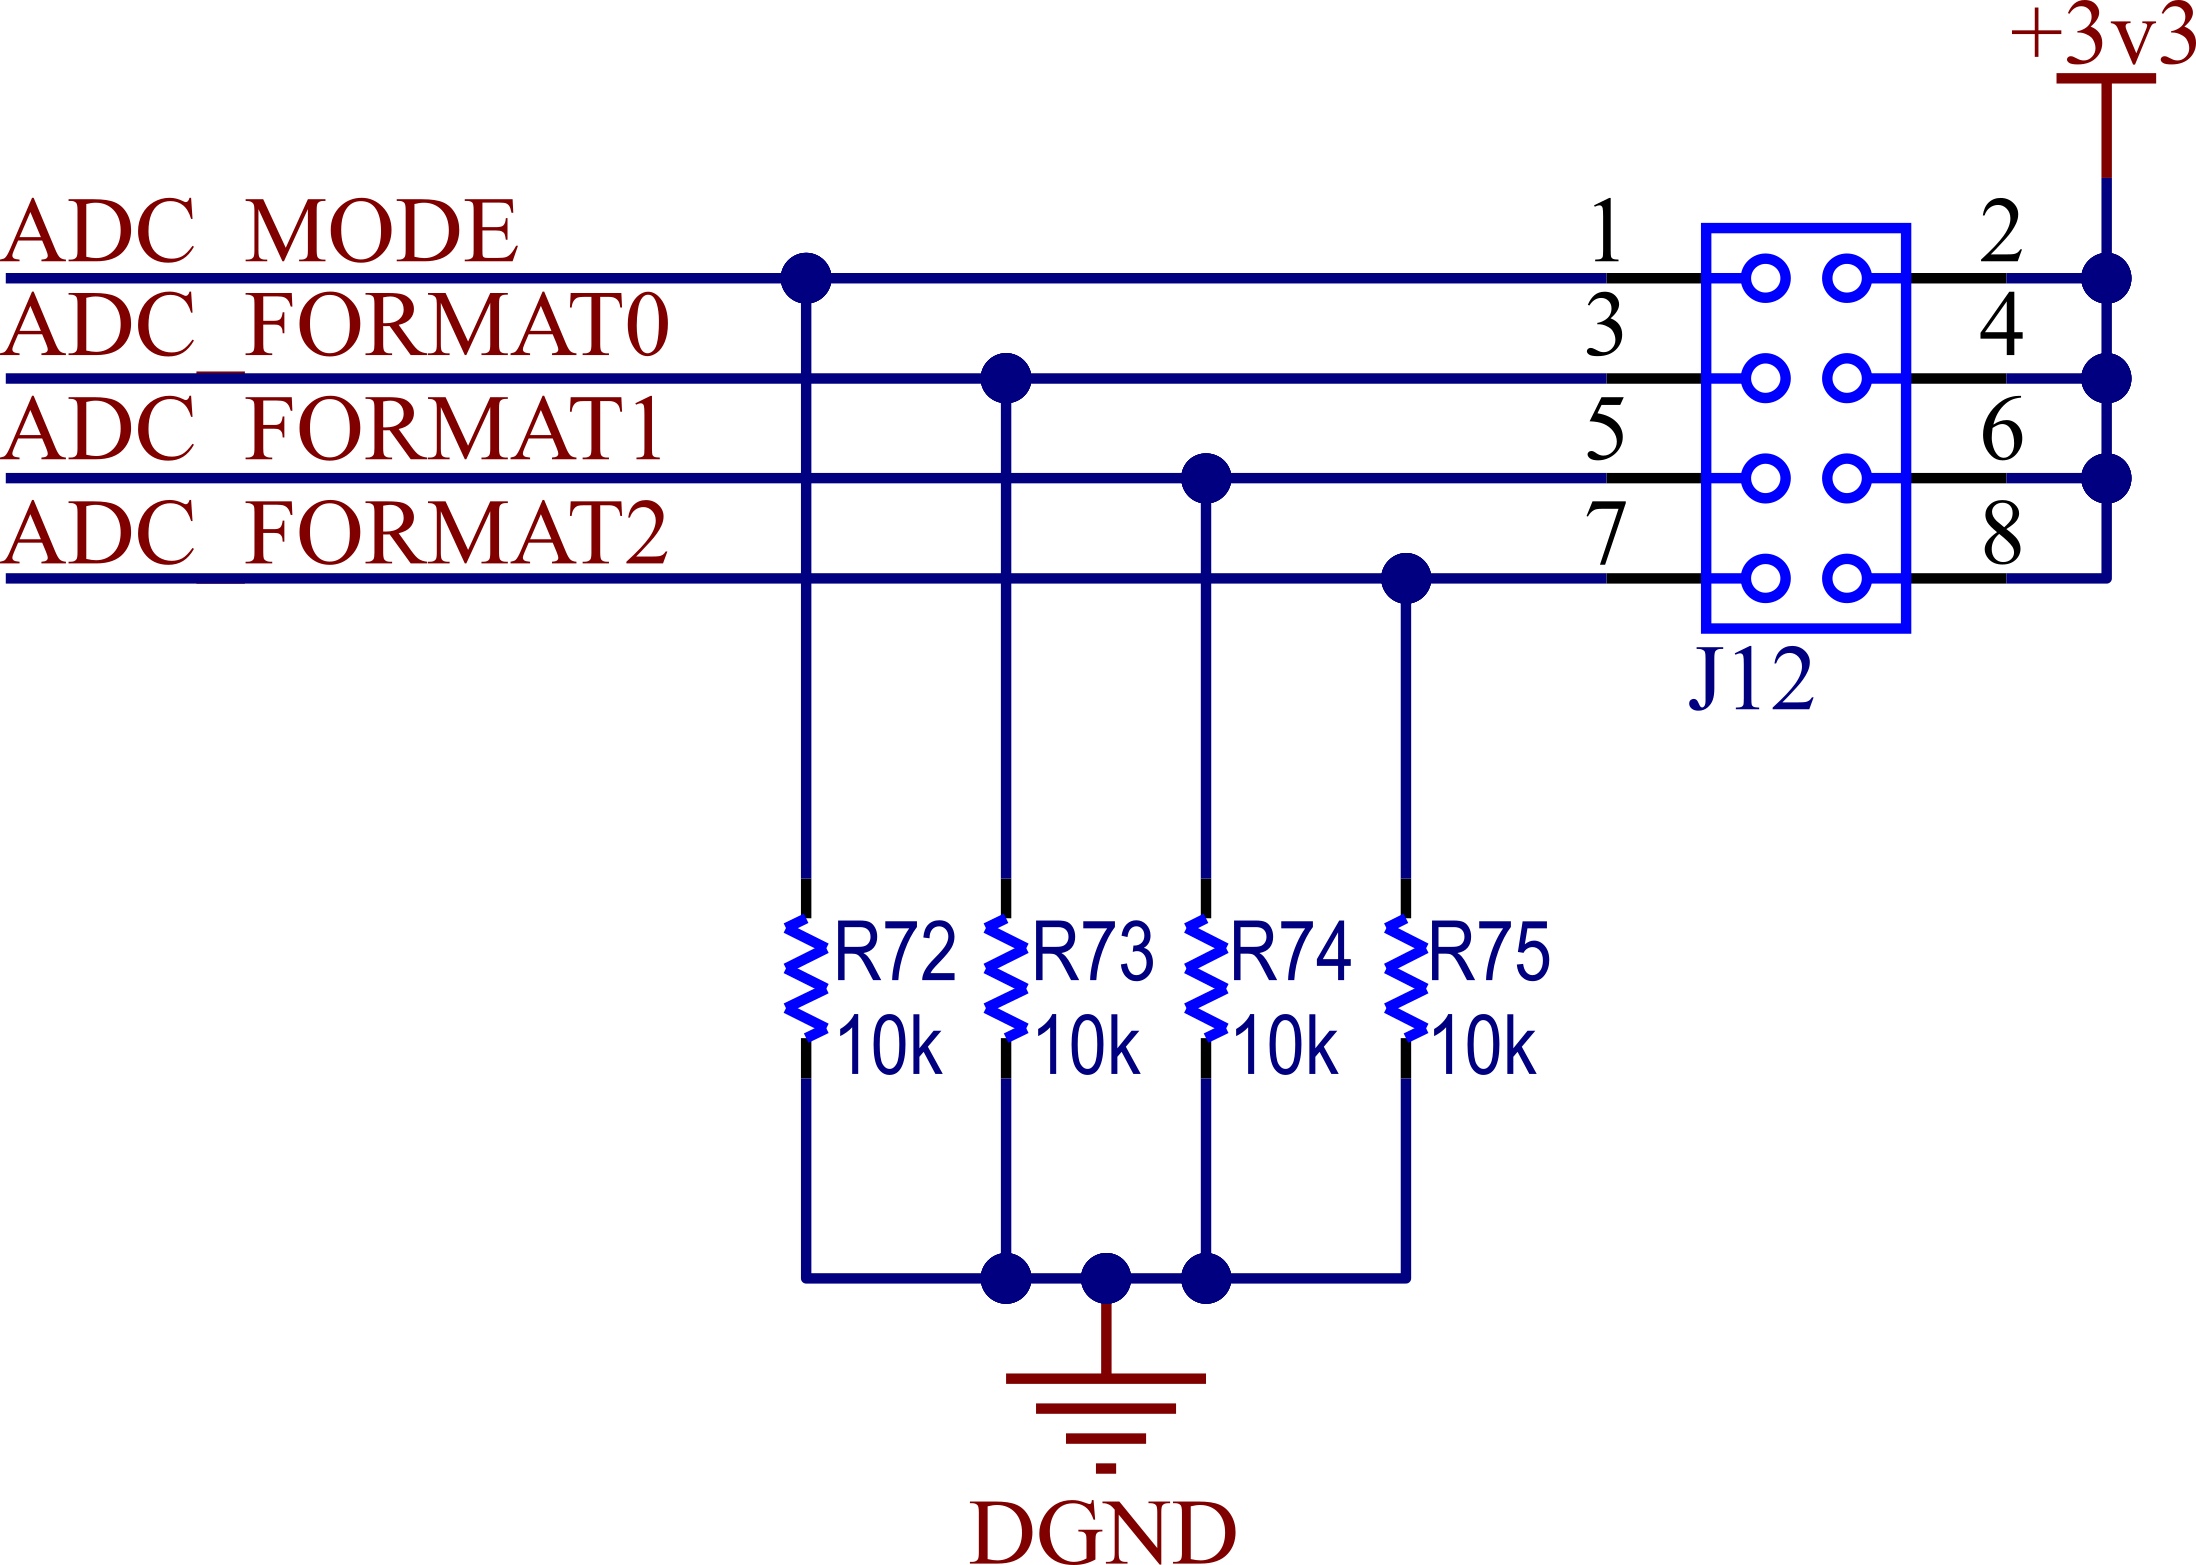
\includegraphics[width=0.4\textwidth]{../images/adc-mode-selector.png}
  \caption{Selector de modo de salida de datos del ADC}
  \label{fig:adc-mode-selector}
\end{figure}

%% ----------------------------------------------------------------
\subsubsection{Modos de testeo}
%% ----------------------------------------------------------------
Este modo permite medir la continudad de los pines de entrada y salida según se ve en la \autoref{tab:adc-test-pins}. Una vez activado, las funciones normales de los pines digitales son deshabilitadas. Nuevamente se dejó un header con pines expuestos en caso de que se necesite utilizar esta función, como se puede ver en la \autoref{fig:adc-test-selector}.

\begin{table}[!htbp]
  \centering
  \begin{tabular}{|c|c|}
    \hline
    \textbf{Entrada}                 & \textbf{Salida}                 \\ \hline
    PWDN1                            & DOUT1                           \\ \hline
    PWDN2                            & DOUT2                           \\ \hline
    PWDN3                            & DOUT3                           \\ \hline
    PWDN4                            & DOUT4                           \\ \hline
    MODE                             & DIN                             \\ \hline
    FORMAT0                          & CLKDIV                          \\ \hline
    FORMAT1                          & DRDY/FSYNC                      \\ \hline
    FORMAT2                          & SCLK                            \\ \hline
  \end{tabular}
  \caption{Conexión interna de pines en modo de testeo del ADC}
  \label{tab:adc-test-pins}
\end{table}

\begin{figure}[!htbp]
  \centering
  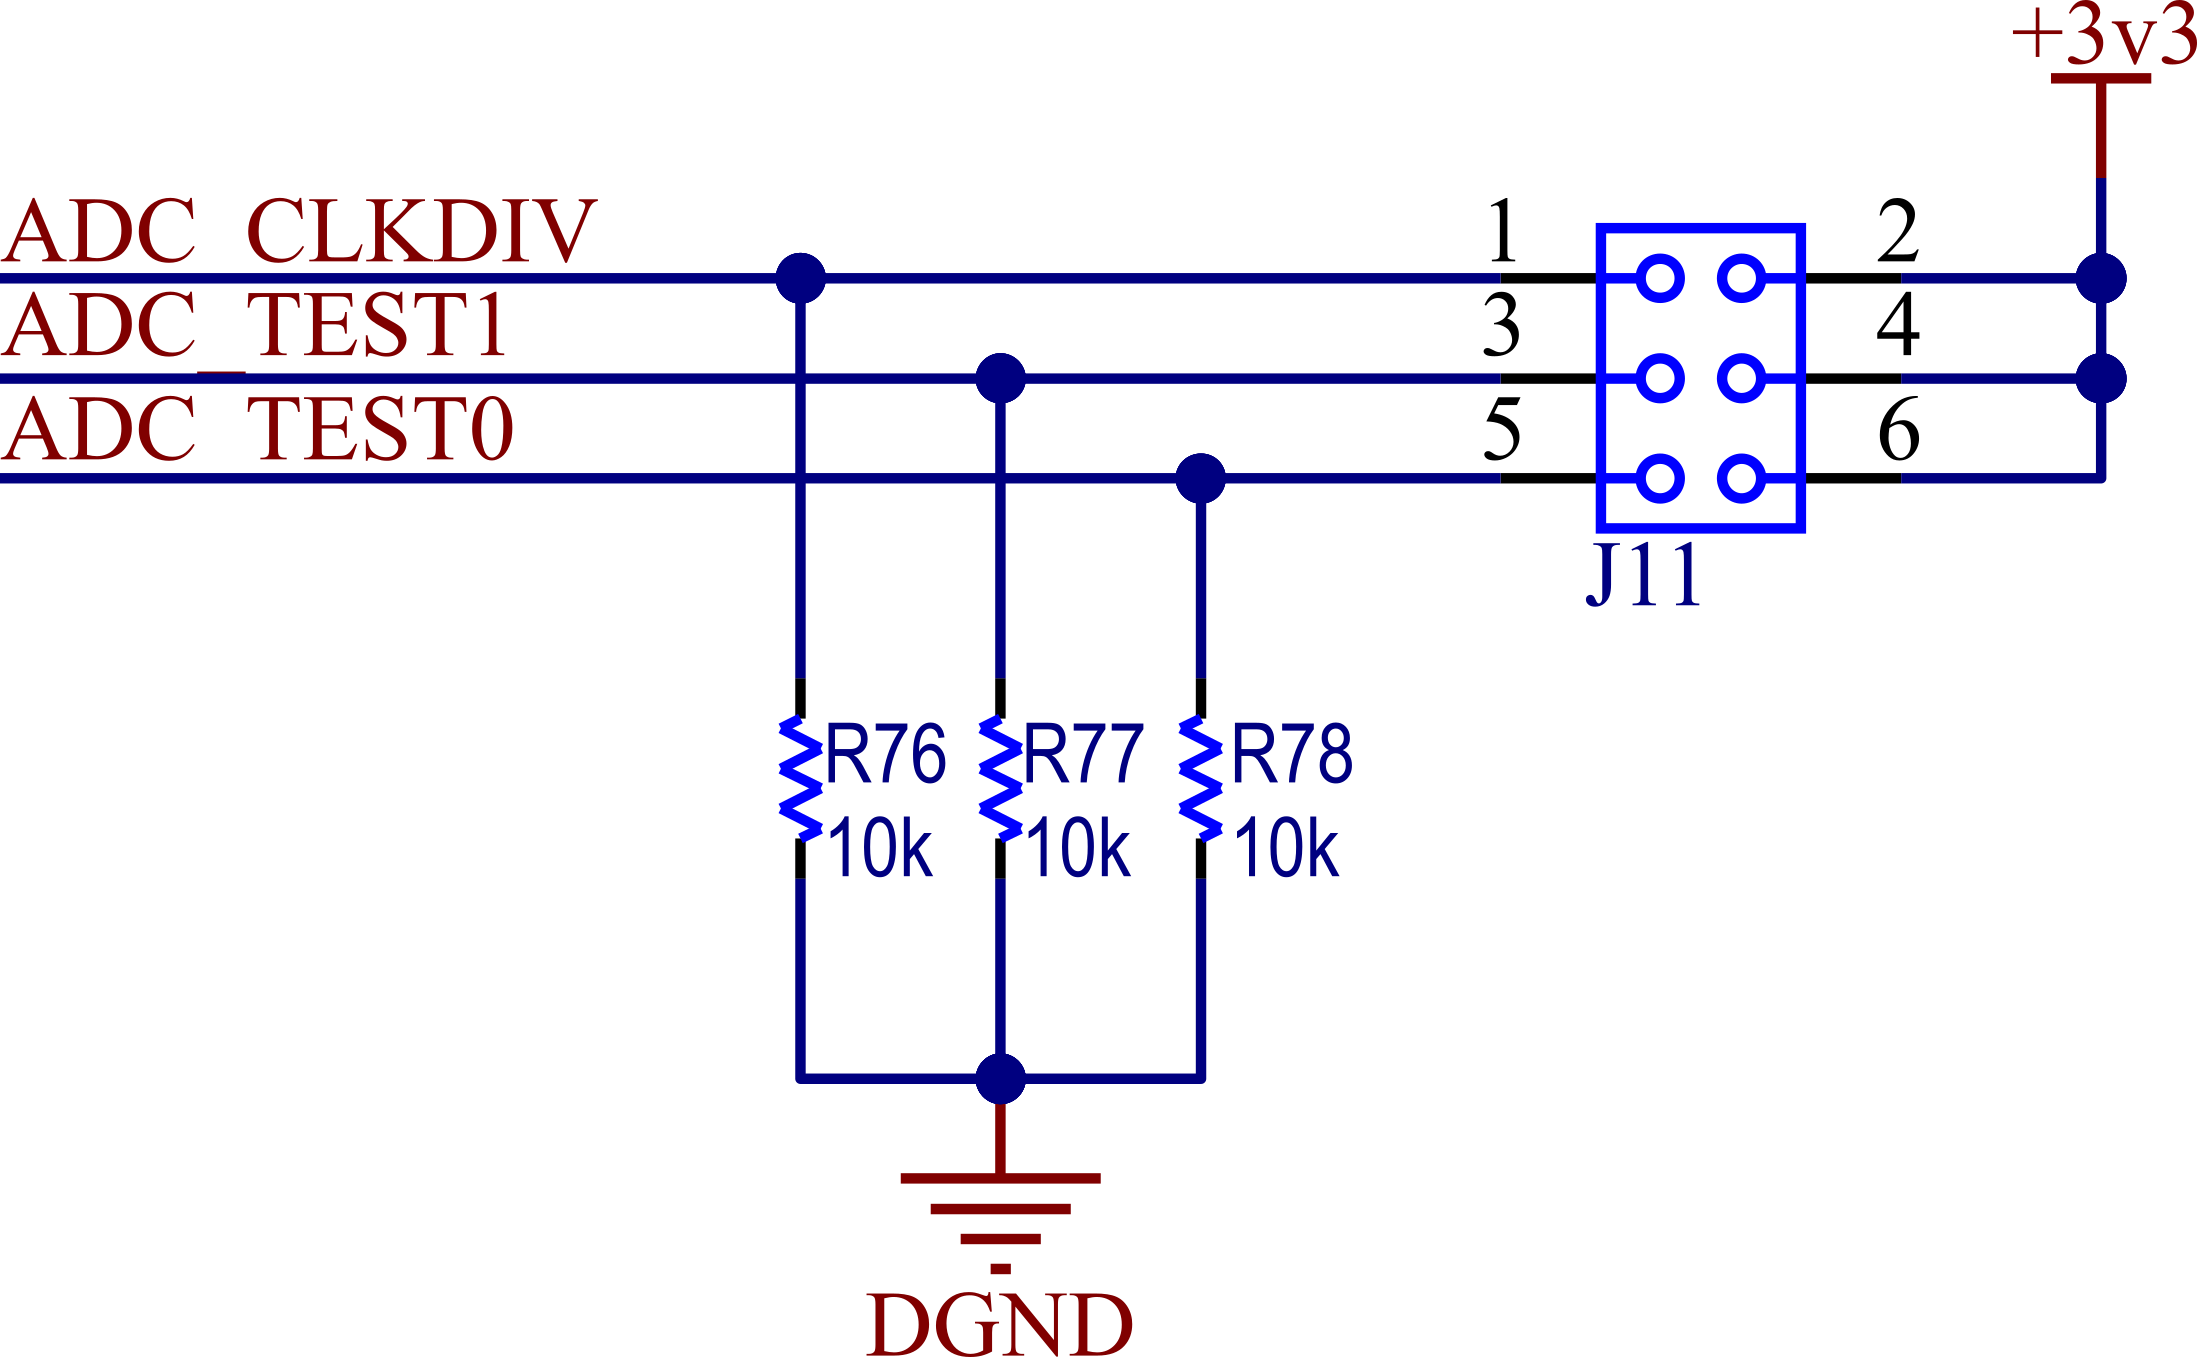
\includegraphics[width=0.5\textwidth]{../images/adc-test-selector.png}
  \caption{Selector de modo de testeo del ADC}
  \label{fig:adc-test-selector}
\end{figure}

%% ----------------------------------------------------------------
\subsubsection{Selección de ADC}
%% ----------------------------------------------------------------
Se contempló el uso del conversor analógico interno del microcontrolador, por lo que se adicionó un header de selección. El esquemático se puede ver en la \autoref{fig:adc-source-selector}.

\begin{figure}[!htbp]
  \centering
  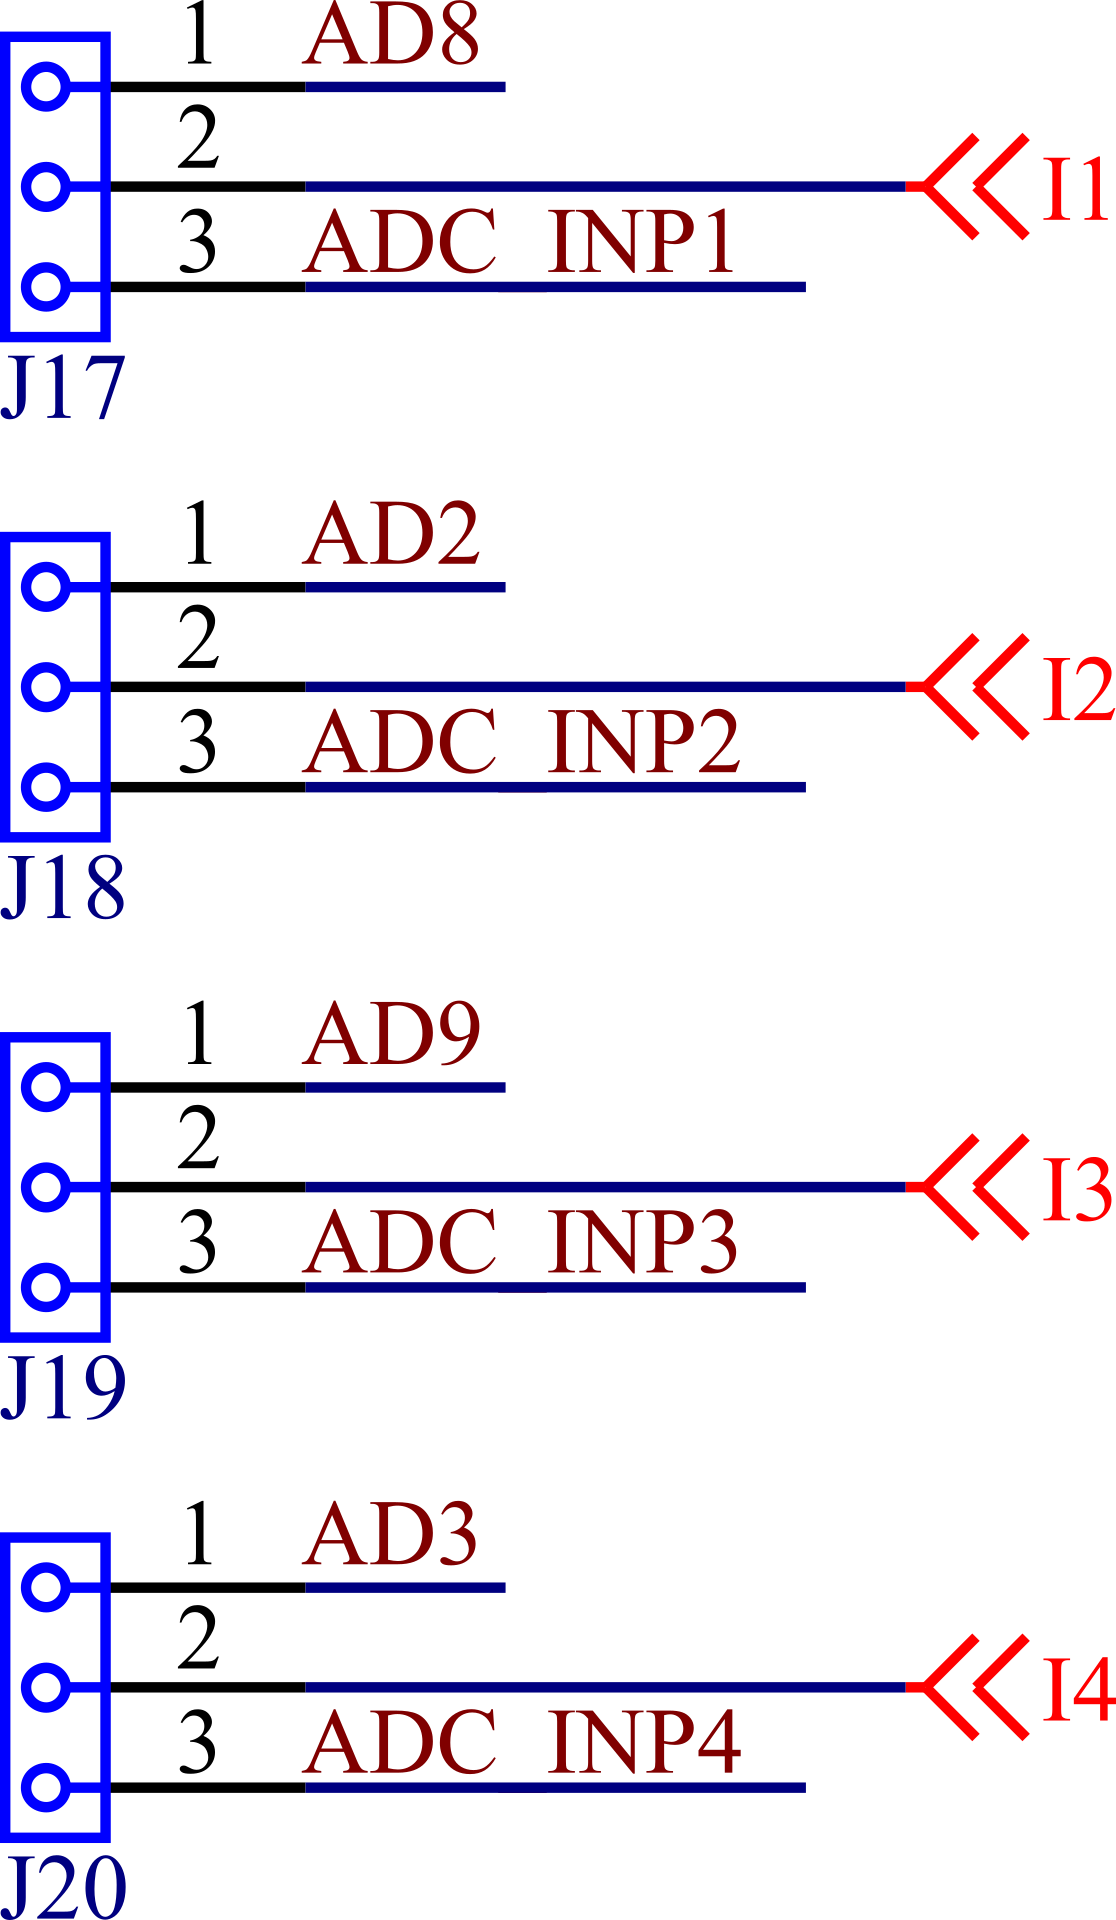
\includegraphics[scale=1.5]{../images/adc-source-selector.png}
  \caption{Selector de ADC}
  \label{fig:adc-source-selector}
\end{figure}

%% ----------------------------------------------------------------
\subsubsection{Características integrado}
%% ----------------------------------------------------------------
El integrado que se utilizará es el ADS1174IPAPT de Analog Devices. Este cuenta con las siguientes características:

\begin{itemize}
  \item 4 canales simultáneos.
  \item Dos modos de selección posibles: \SI{52}{kSPS} o \SI{10}{kSPS}.
  \item DC Performance:
    \begin{itemize}
      \item \SI{2}{\micro V/\degree C} deriva de offset
      \item \SI{2}{ppm/\degree C} deriva de ganancia
    \end{itemize}

    \item AC Performance:
      \begin{itemize}
        \item \SI{25}{kHz} de ancho de banda
        \item \SI{97}{dB} de SNR
        \item \SI{-105}{dB} de THD
      \end{itemize}
  \item Interfaz SPI.
  \item Muestreador tipo delta-sigma.
  \item Filtro interno de \SI{\pm 0.005}{dB} de ripple y respuesta de fase lineal.
\end{itemize}

En la \autoref{fig:adc-bloques} se puede observar el diagrama en bloques interno del integrado, provisto por el fabricante.

\begin{figure}[!htbp]
  \centering
  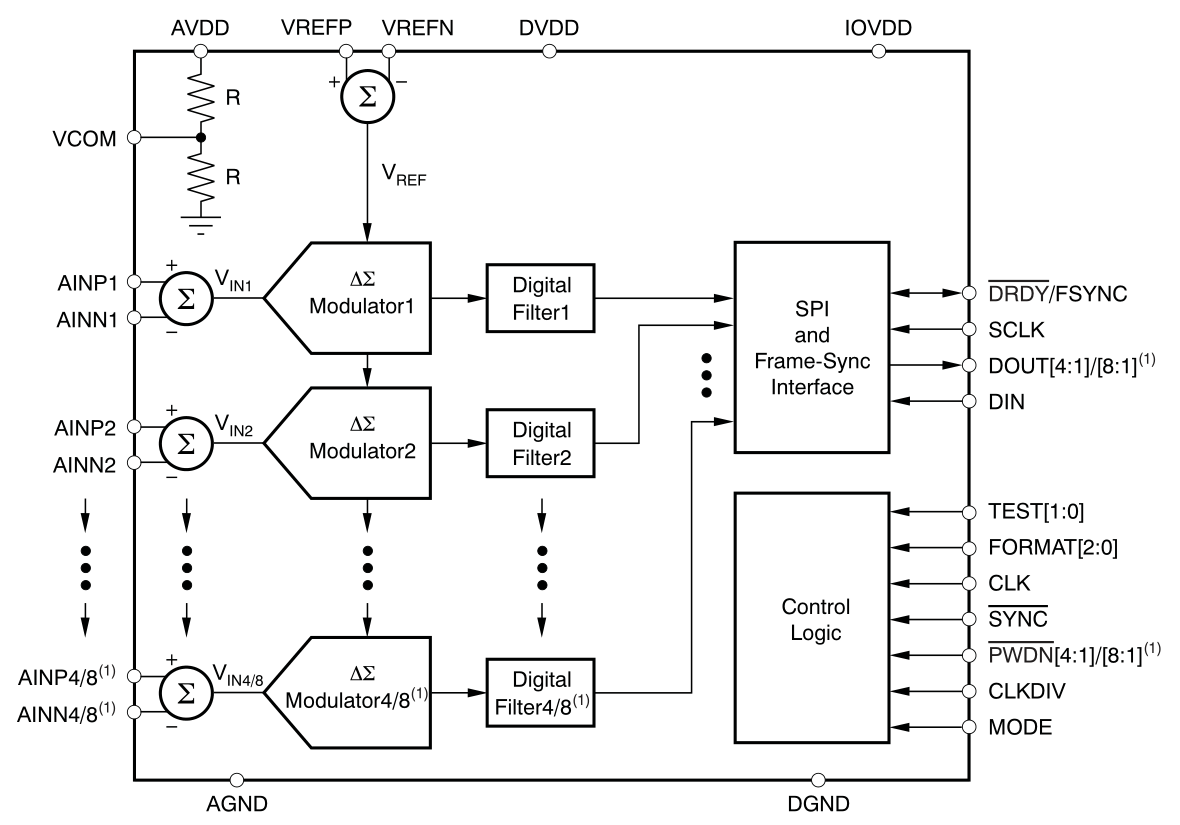
\includegraphics[scale=0.4]{../images/adc-bloques.png}
  \caption{Diagrama en bloques interno del ADS1174IPAPT}
  \label{fig:adc-bloques}
\end{figure}


\end{document}